% Source PDF page 335 (printed p. 321)
稳健逼近问题 (6.14) 出现在许多场合和应用中。在估计问题中，集合 $\mathcal A$ 描述待估向量与测量向量之间线性关系的不确定性。模型 $y=Ax+v$ 中的噪声项 $v$ 有时称为\emph{加性噪声}或\emph{加性误差}，因为它加在“理想”测量 $Ax$ 上。相对地，$A$ 的变化称为\emph{乘性误差}，因为它与变量 $x$ 相乘。

在最优设计中，这种变化可以表示连接设计变量 $x$ 与结果向量 $Ax$ 的线性方程的不确定性，例如来自制造过程的不确定性。此时，稳健逼近问题 (6.14) 就解释为稳健设计问题：寻找设计变量 $x$，使对所有可能的 $A$ 而言，$Ax$ 与 $b$ 之间可能出现的最大偏差最小。

\subsubsection*{有限集合}
此时 $\mathcal A=\{A_1,\ldots,A_k\}$，稳健逼近问题为
\[\text{最小化}\quad\max_{i=1,\ldots,k}\norm{A_ix-b}.\]
它等价于采用多面体集合 $\mathcal A=\conv\{A_1,\ldots,A_k\}$ 的稳健逼近问题：
\[\text{最小化}\quad\sup\{\norm{Ax-b}\mid A\in\conv\{A_1,\ldots,A_k\}\}.\]
问题可以写成上图形式
\[\begin{array}{ll}\text{最小化}&t\\\text{约束条件}&\norm{A_ix-b}\le t,\quad i=1,\ldots,k.\end{array}\]
根据所用范数的不同，可以有多种求解方法。若采用欧几里得范数，它就是 SOCP；若采用 $\ell_1$ 或 $\ell_\infty$ 范数，则可以写成 LP。

\subsubsection*{范数有界误差}
这里不确定集 $\mathcal A$ 是一个范数球：$\mathcal A=\{\overline A+U\mid\norm U\le a\}$，其中 $\norm{\cdot}$ 是 $\R^{m\times n}$ 上的范数。于是
\[e_{\rm wc}(x)=\sup\{\norm{\overline Ax-b+Ux}\mid\norm U\le a\}.\]
需要仔细理解该式：第一个范数定义在 $\R^m$ 上，用于衡量残差大小；第二个范数定义在 $\R^{m\times n}$ 上，用于定义范数球 $\mathcal A$。

在若干情形下，$e_{\rm wc}(x)$ 的这一表达式可以简化。例如，在 $\R^n$ 上采用欧几里得范数，在 $\R^{m\times n}$ 上采用相应的诱导范数，即最大奇异值。如果 $\overline Ax-b\ne0$ 且 $x\ne0$，那么 $e_{\rm wc}(x)$ 中的上确界在 $U=auv^\T$ 处取得，其中
\[u=\frac{\overline Ax-b}{\norm{\overline Ax-b}_2},\qquad v=\frac x{\norm x_2},\]
从而最坏情形误差为
\[e_{\rm wc}(x)=\norm{\overline Ax-b}_2+a\norm x_2.\]

% Source PDF page 336 (printed p. 322)
（容易验证，$x$ 或 $\overline Ax-b$ 为零时，这一表达式同样成立。）稳健逼近问题 (6.14) 因此变成
\[\text{最小化}\quad\norm{\overline Ax-b}_2+a\norm x_2,\]
这是一个正则化范数问题，可以写成 SOCP
\[\begin{array}{ll}\text{最小化}&t_1+at_2\\\text{约束条件}&\norm{\overline Ax-b}_2\le t_1,\quad\norm x_2\le t_2.\end{array}\]
对某个正则化参数 $\delta$，该问题的解与正则化最小二乘问题
\[\text{最小化}\quad\norm{\overline Ax-b}_2^2+\delta\norm x_2^2\]
的解相同，因此又得到了将正则化最小二乘问题解释为最坏情形稳健逼近问题的一种方式。

\subsubsection*{不确定性椭球}
也可以为 $A$ 的每一行给出一个可能取值的椭球，以描述 $A$ 的变化：
\[\mathcal A=\{[a_1\ \cdots\ a_m]^\T\mid a_i\in\mathcal E_i,\ i=1,\ldots,m\},\]
其中
\[\mathcal E_i=\{\overline a_i+P_i u\mid\norm u_2\le1\}.\]
矩阵 $P_i\in\R^{n\times n}$ 描述 $a_i$ 的变化。允许 $P_i$ 具有非平凡零空间，以刻画 $a_i$ 的变化局限于某个子空间的情形。极端情况下，若 $a_i$ 没有不确定性，就取 $P_i=0$。

在这种椭球不确定性描述下，每个残差幅度的最坏值有显式表达式：
\[\begin{aligned}
\sup_{a_i\in\mathcal E_i}|a_i^\T x-b_i|
&=\sup\{|\overline a_i^\T x-b_i+(P_iu)^\T x|\mid\norm u_2\le1\}\\
&=|\overline a_i^\T x-b_i|+\norm{P_i^\T x}_2.
\end{aligned}\]
利用这一结果，可以求解若干稳健逼近问题。例如，稳健 $\ell_2$ 范数逼近问题
\[\text{最小化}\quad e_{\rm wc}(x)=\sup\{\norm{Ax-b}_2\mid a_i\in\mathcal E_i,\ i=1,\ldots,m\}\]
可以按以下方式化为 SOCP。最坏情形误差的显式表达式为
\[\begin{aligned}
e_{\rm wc}(x)&=\left(\sum_{i=1}^m\sup_{a_i\in\mathcal E_i}|a_i^\T x-b_i|^2\right)^{1/2}\\
&=\left(\sum_{i=1}^m\bigl(|\overline a_i^\T x-b_i|+\norm{P_i^\T x}_2\bigr)^2\right)^{1/2}.
\end{aligned}\]
为了最小化 $e_{\rm wc}(x)$，可以求解
\[\begin{array}{ll}\text{最小化}&\norm t_2\\\text{约束条件}&|\overline a_i^\T x-b_i|+\norm{P_i^\T x}_2\le t_i,\quad i=1,\ldots,m,\end{array}\]
其中引入了新变量 $t_1,\ldots,t_m$。

% Source PDF page 337 (printed p. 323)
该问题可以表述为
\[\begin{array}{ll}\text{最小化}&\norm t_2\\\text{约束条件}&\overline a_i^\T x-b_i+\norm{P_i^\T x}_2\le t_i,\quad i=1,\ldots,m,\\&-\overline a_i^\T x+b_i+\norm{P_i^\T x}_2\le t_i,\quad i=1,\ldots,m,\end{array}\]
写成上图形式后就成为 SOCP。

\subsubsection*{具有线性结构的范数有界误差}
作为范数有界描述 $\mathcal A=\{\overline A+U\mid\norm U\le a\}$ 的推广，可以将 $\mathcal A$ 定义为一个范数球在仿射变换下的像：
\[\mathcal A=\{\overline A+u_1A_1+u_2A_2+\cdots+u_pA_p\mid\norm u\le1\},\]
其中 $\norm{\cdot}$ 是 $\R^p$ 上的范数，$p+1$ 个矩阵 $\overline A,A_1,\ldots,A_p\in\R^{m\times n}$ 已知。最坏情形误差可写为
\[\begin{aligned}
e_{\rm wc}(x)&=\sup_{\norm u\le1}\norm{(\overline A+u_1A_1+\cdots+u_pA_p)x-b}\\
&=\sup_{\norm u\le1}\norm{P(x)u+q(x)},
\end{aligned}\]
其中 $P$ 和 $q$ 定义为
\[P(x)=[A_1x\ A_2x\ \cdots\ A_px]\in\R^{m\times p},\qquad q(x)=\overline Ax-b\in\R^m.\]
先考虑稳健 Chebyshev 逼近问题
\[\text{最小化}\quad e_{\rm wc}(x)=\sup_{\norm u_\infty\le1}\norm{(\overline A+u_1A_1+\cdots+u_pA_p)x-b}_\infty.\]
此时可以导出最坏情形误差的显式表达式。令 $p_i(x)^\T$ 为 $P(x)$ 的第 $i$ 行，有
\[\begin{aligned}
e_{\rm wc}(x)&=\sup_{\norm u_\infty\le1}\norm{P(x)u+q(x)}_\infty\\
&=\max_{i=1,\ldots,m}\sup_{\norm u_\infty\le1}|p_i(x)^\T u+q_i(x)|\\
&=\max_{i=1,\ldots,m}\bigl(\norm{p_i(x)}_1+|q_i(x)|\bigr).
\end{aligned}\]
因此，稳健 Chebyshev 逼近问题可以写为 LP
\[\begin{array}{ll}\text{最小化}&t\\\text{约束条件}&-y_0\preceq\overline Ax-b\preceq y_0,\\&-y_k\preceq A_kx\preceq y_k,\quad k=1,\ldots,p,\\&y_0+\displaystyle\sum_{k=1}^p y_k\preceq t\one,\end{array}\]
变量为 $x\in\R^n$、$y_k\in\R^m$、$t\in\R$。

再考虑稳健最小二乘问题
\[\text{最小化}\quad e_{\rm wc}(x)=\sup_{\norm u_2\le1}\norm{(\overline A+u_1A_1+\cdots+u_pA_p)x-b}_2.\]

% Source PDF page 338 (printed p. 324)
这里使用拉格朗日对偶来计算 $e_{\rm wc}$。最坏情形误差 $e_{\rm wc}(x)$ 是如下非凸二次优化问题最优值的平方根：
\[\begin{array}{ll}\text{最大化}&\norm{P(x)u+q(x)}_2^2\\\text{约束条件}&u^\T u\le1,\end{array}\]
变量为 $u$。这个问题的拉格朗日对偶可以写成 SDP
\begin{equation}
\begin{array}{ll}\text{最小化}&t+\lambda\\\text{约束条件}&\begin{bmatrix}I&P(x)&q(x)\\P(x)^\T&\lambda I&0\\q(x)^\T&0&t\end{bmatrix}\succeq0,\end{array}\tag{6.15}
\end{equation}
变量为 $t,\lambda\in\R$。而且，正如第5.2节与第B.1节提到（并在第B.4节证明）的，这一对原问题与对偶问题满足强对偶。换言之，固定 $x$ 后，通过求解以 $t$、$\lambda$ 为变量的 SDP (6.15)，就能计算 $e_{\rm wc}(x)^2$。联合优化 $t$、$\lambda$ 和 $x$，等价于最小化 $e_{\rm wc}(x)^2$。因此，稳健最小二乘问题等价于以 $x$、$\lambda$、$t$ 为变量的 SDP (6.15)。

\begin{origexample}{6.6}
\emph{最坏情形稳健解、Tikhonov 正则化解与标称最小二乘解的比较。}考虑稳健逼近问题的一个实例：
\begin{equation}
\text{最小化}\quad\sup_{\norm u_2\le1}\norm{(\overline A+u_1A_1+u_2A_2)x-b}_2,\tag{6.16}
\end{equation}
维数为 $m=50$、$n=20$。矩阵 $\overline A$ 的范数为 $10$，矩阵 $A_1$、$A_2$ 的范数均为 $1$，因此粗略地说，矩阵 $A$ 的变化约为 $10\%$。不确定参数 $u_1$、$u_2$ 位于 $\R^2$ 的单位圆盘内。

计算稳健最小二乘问题 (6.16) 的最优解 $x_{\rm rls}$，以及标称最小二乘问题的解 $x_{\rm ls}$（即假定 $u=0$），还计算 $\delta=1$ 的 Tikhonov 正则化解 $x_{\rm tik}$。

为说明各个近似解对参数 $u$ 的敏感性，生成 $10^5$ 个在单位圆盘内均匀分布的参数向量，并对每个参数值计算残差
\[\norm{(A_0+u_1A_1+u_2A_2)x-b}_2.\]
残差分布见图6.16。

可以作出几点观察。首先，标称最小二乘解的残差分布很宽，从约 $0.52$ 的最小值到约 $4.9$ 的最大值。特别地，最小二乘解对参数变化非常敏感。相反，当不确定参数在单位圆盘内变化时，稳健最小二乘解和 Tikhonov 正则化解的残差变化小得多。例如，稳健最小二乘解在单位圆盘内所有参数下的残差都介于 $2.0$ 与 $2.6$ 之间。
\end{origexample}

\section{函数拟合与插值}
函数拟合问题要从一个有限维函数子空间中选择一个函数，使其最好地满足给定的数据或要求。为简便起见，只考虑实值函数；这些想法也容易扩展到向量值函数。

% Source PDF page 339 (printed p. 325)
\begin{figure}[htbp]\centering
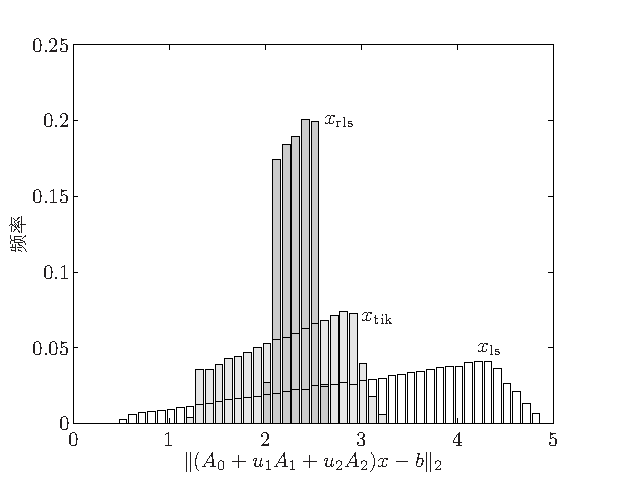
\includegraphics[width=.72\textwidth]{ch06-16.pdf}
\caption*{图6.16\quad 最小二乘问题 (6.16) 的三个解所对应的残差分布：$x_{\rm ls}$ 是假定 $u=0$ 的最小二乘解；$x_{\rm tik}$ 是 $\delta=1$ 的 Tikhonov 正则化解；$x_{\rm rls}$ 是稳健最小二乘解。这些直方图通过从 $\R^2$ 单位圆盘上的均匀分布中生成 $10^5$ 个不确定参数向量 $u$ 得到，分箱宽度为 $0.1$。}
\end{figure}

% Source PDF page 340 (printed p. 326)
\subsection{函数族}
考虑函数族 $f_1,\ldots,f_n:\R^k\to\R$，它们具有共同定义域 $\dom f_i=\mathcal D$。对每个 $x\in\R^n$，关联函数 $f:\R^k\to\R$，定义为
\begin{equation}f(u)=x_1f_1(u)+\cdots+x_nf_n(u),\tag{6.17}\end{equation}
且 $\dom f=\mathcal D$。即使函数不线性无关，函数族 $\{f_1,\ldots,f_n\}$ 有时也称为拟合问题的\emph{基函数}集。将函数子空间参数化的向量 $x\in\R^n$ 是优化变量，有时称为\emph{系数向量}。这些基函数生成 $\mathcal D$ 上的函数子空间 $\mathcal F$。

在许多应用中，会利用先验知识或经验专门选择基函数，以便用有限维函数子空间合理地描述所关心的函数。另一些情况下，则采用更通用的函数族。下面介绍其中几种。

\subsubsection*{多项式}
$\R$ 上的一个常用函数子空间，是次数小于 $n$ 的多项式空间。最简单的基由幂函数构成，即 $f_i(t)=t^{i-1}$，$i=1,\ldots,n$。许多应用中，会用另一组基描述同一子空间；例如采用次数小于 $n$ 的一组多项式 $f_1,\ldots,f_n$，使它们关于某个正函数（或测度）$\phi:\R^n\to\R_+$ 正交归一，即
\[\int f_i(t)f_j(t)\phi(t)\,dt=\begin{cases}1,&i=j,\\0,&i\ne j.\end{cases}\]
另一组常用多项式基，是与互异点 $t_1,\ldots,t_n$ 对应的 Lagrange 基 $f_1,\ldots,f_n$，满足
\[f_i(t_j)=\begin{cases}1,&i=j,\\0,&i\ne j.\end{cases}\]
也可以考虑 $\R^k$ 上的多项式，限制其最大总次数，或每个变量的最高次数。

一个相关例子是次数小于 $n$ 的三角多项式，其基为
\[\sin kt,\quad k=1,\ldots,n-1,\qquad\cos kt,\quad k=0,\ldots,n-1.\]

\subsubsection*{分段线性函数}
先对定义域 $\mathcal D$ 作三角剖分，其含义如下。给定一组网格点 $g_1,\ldots,g_n\in\R^k$，并将 $\mathcal D$ 划分为一组单纯形：
\[\mathcal D=S_1\cup\cdots\cup S_m,\qquad\operatorname{int}(S_i\cap S_j)=\varnothing\quad(i\ne j).\]
每个单纯形是 $k+1$ 个网格点的凸包，而且要求：一个网格点若属于某个单纯形，就必须是它的顶点。

% Source PDF page 341 (printed p. 327)
\begin{figure}[htbp]\centering
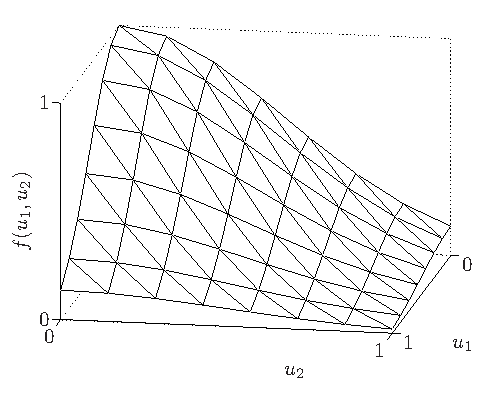
\includegraphics[width=.64\textwidth]{ch06-17.pdf}
\caption*{图6.17\quad 单位正方形上的二元分段线性函数。三角剖分由单位正方形内的64个均匀网格点和98个单纯形构成。}
\end{figure}
给定三角剖分后，可以先给网格点赋函数值 $f(g_i)=x_i$，再在每个单纯形上作仿射延拓，构造分段线性函数（更准确地说，分段仿射函数）$f$。函数 $f$ 可写为式 (6.17)，其中基函数 $f_i$ 在每个单纯形上仿射，并由下述条件定义：
\[f_i(g_j)=\begin{cases}1,&i=j,\\0,&i\ne j.\end{cases}\]
按这种构造得到的函数是连续的。

图6.17给出了 $k=2$ 的一个例子。

\subsubsection*{分段多项式与样条}
三角剖分定义域上的分段仿射函数这一想法，容易推广到分段多项式和其他函数。

分段多项式在三角剖分的每个单纯形上定义为某个最高次数以下的多项式，并且是连续的，即相邻单纯形上的多项式在公共边界处取值一致。进一步要求分段多项式直到某一阶的导数连续，就可以定义各种样条函数。图6.18是三次样条的例子，即 $\R$ 上一阶、二阶导数连续的三次分段多项式。

% Source PDF page 342 (printed p. 328)
\begin{figure}[htbp]\centering
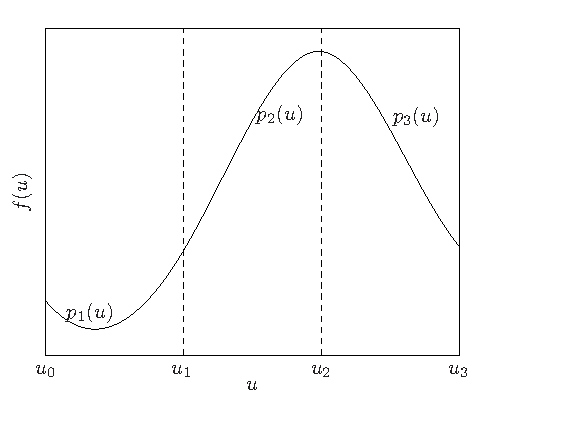
\includegraphics[width=.65\textwidth]{ch06-18.pdf}
\caption*{图6.18\quad 三次样条。三次样条是具有连续一阶、二阶导数的分段多项式。本例中，三次样条 $f$ 由三个三次多项式构成：$p_1$ 定义在 $[u_0,u_1]$，$p_2$ 定义在 $[u_1,u_2]$，$p_3$ 定义在 $[u_2,u_3]$。相邻多项式在边界点 $u_1$、$u_2$ 处函数值相等，一阶、二阶导数也相等。本例中函数族的维数为 $n=6$，因为有12个多项式系数（每个三次多项式4个），以及6个等式约束（$u_1$、$u_2$ 处各3个）。}
\end{figure}

% Source PDF page 343 (printed p. 329)
\subsection{约束}
本节介绍可以施加在函数 $f$ 上、从而施加在变量 $x\in\R^n$ 上的一些约束。

\subsubsection*{函数值插值与不等式}
令 $v$ 为 $\mathcal D$ 中的一点。$f$ 在 $v$ 的值
\[f(v)=\sum_{i=1}^n x_i f_i(v)\]
是 $x$ 的线性函数。因此，要求函数 $f$ 在指定点 $v_j\in\mathcal D$ 处取指定值 $z_j\in\R$ 的插值条件
\[f(v_j)=z_j,\qquad j=1,\ldots,m,\]
构成关于 $x$ 的一组线性等式。更一般地，对给定点函数值的不等式要求，如 $l\le f(v)\le u$，也是关于变量 $x$ 的线性不等式。还有许多涉及有限点集 $v_1,\ldots,v_N$ 上函数值的有意义的凸约束。例如，Lipschitz 约束
\[|f(v_j)-f(v_k)|\le L\norm{v_j-v_k},\qquad j,k=1,\ldots,m,\]
构成关于 $x$ 的一组线性不等式。

也可以对无穷多个点上的函数值施加不等式。例如，考虑非负约束
\[f(u)\ge0\quad\text{对所有 }u\in\mathcal D.\]
这是关于 $x$ 的凸约束，因为它是无穷多个半空间的交；但除非利用函数特殊结构的某些情形，否则未必得到可处理的问题。一个简单例子是分段线性函数：如果网格点处的函数值非负，函数就处处非负，因此只需一组简单的有限线性不等式。

再看一个不那么简单的例子。考虑 $\R$ 上最高次数为偶数 $2k$ 的多项式，即 $n=2k+1$，并令 $\mathcal D=\R$。如第65页习题2.37所示，非负约束
\[p(u)=x_1+x_2u+\cdots+x_{2k+1}u^{2k}\ge0\quad\text{对所有 }u\in\R\]
等价于
\[x_i=\sum_{m+n=i+1}Y_{mn},\quad i=1,\ldots,2k+1,\qquad Y\succeq0,\]
其中 $Y\in\mathbf S^{k+1}$ 是辅助变量。

% Source PDF page 344 (printed p. 330)
\subsubsection*{导数约束}
假设基函数 $f_i$ 在点 $v\in\mathcal D$ 可微。梯度
\[\nabla f(v)=\sum_{i=1}^n x_i\nabla f_i(v)\]
是 $x$ 的线性函数，因此对 $f$ 在 $v$ 处导数的插值条件，可化为关于 $x$ 的线性等式约束。要求 $v$ 处梯度的范数不超过给定上限，
\[\norm{\nabla f(v)}=\left\|\sum_{i=1}^n x_i\nabla f_i(v)\right\|\le M,\]
是关于 $x$ 的凸约束。同样的想法也适用于高阶导数。例如，如果 $f$ 在 $v$ 二阶可微，则要求
\[lI\preceq\nabla^2f(v)\preceq uI\]
是关于 $x$ 的线性矩阵不等式，因此为凸约束。

也可以对无穷多个点处的导数施加约束。例如，要求 $f$ 单调：
\[f(u)\ge f(v)\quad\text{对所有 }u,v\in\mathcal D,\ u\succeq v.\]
这是关于 $x$ 的凸约束，但除某些特殊情形外，未必得到可处理的问题。例如，当 $f$ 分段仿射时，单调性约束等价于每个单纯形内部有 $\nabla f(v)\succeq0$。由于梯度是网格点取值的线性函数，这就得到一组简单的有限线性不等式。

另一个例子是要求函数为凸函数，即满足
\[f((u+v)/2)\le(f(u)+f(v))/2\quad\text{对所有 }u,v\in\mathcal D\]
（$f$ 连续时，这足以保证凸性）。这是一个凸约束，在某些情况下具有可处理的表示。一个明显的例子是 $f$ 为二次函数，此时凸性约束等价于要求 $f$ 的二次部分非负，这就是一个 LMI。第6.5.5节将更详细地介绍另一个凸性约束产生可处理问题的例子。

\subsubsection*{积分约束}
函数子空间上的任意线性泛函 $L$ 都可表示为 $x$ 的线性函数，即 $L(f)=c^\T x$。在某点求 $f$ 或其导数的值，只是一个特例。另一个例子是线性泛函
\[L(f)=\int_{\mathcal D}\phi(u)f(u)\,du,\]
